\documentclass{beamer}
%--------------------------------------------------------------------------------------------------%
%--------------------------------------------------------------------------------------------------%
% Preamble
% Load Packages
\usepackage{etex}
\usepackage{xcolor}
\usepackage{tikz}
%\usetikzlibrary{matrix, arrows, positioning}
\usepackage{amsmath}
\usepackage{amssymb}
\usepackage{here}
\usepackage{graphicx}
\usepackage{epstopdf}
\usepackage{framed}
\usepackage{stmaryrd}
\usepackage{amsthm}
\usepackage{multicol}
\usepackage{fancybox}
\usepackage{pdflscape}
\usepackage{epsfig}
\usepackage{multirow}
\usepackage{color}
\usepackage{booktabs}
\usepackage{natbib}
\usepackage{lettrine}
\usepackage{appendix}
\usepackage{ifthen}
\usepackage[affil-it]{authblk}
\usepackage[flushleft]{threeparttable}

\newcommand{\sym}[1]{{$#1$}}

\definecolor{darkblue}{rgb}{0,0,0.5451}

%\usepackage{tikz-cd}

% Define Layout
\usetheme{CambridgeUS}
\usecolortheme{rose}
\useinnertheme{default}
\useoutertheme{default}
\usefonttheme{serif}

% Define item symbol
\setbeamertemplate{itemize items}[circle]

% Transparente Overlays
% \setbeamercovered{transparent}

% Deactivate Navigationssymbols
\beamertemplatenavigationsymbolsempty

% Add Frame Number
\setbeamertemplate{footline}[frame number]

% Define Titlepage
\title{The political economy of European asylum policies}
\subtitle{\small\textcolor{black}{Marcus Drometer, Martina Burmann and Romuald M\'eango\\[1ex]
\scriptsize{\hspace{10ex}Ifo Institute \hspace{29ex} MEA}}}\date{12 December 2017\\[3ex]
{ifo Christmas Conference\\[3ex]
%\newline Location
}}
% End Preamble
%--------------------------------------------------------------------------------------------------%
%--------------------------------------------------------------------------------------------------%
\begin{document}
%--------------------------------------------------------------------------------------------------%
	\begin{frame}
\titlepage
	\end{frame}
%--------------------------------------------------------------------------------------------------%
\section{Introduction}
%--------------------------------------------------------------------------------------------------%
	\begin{frame}{Why is the research question interesting?}
Dustmann (2016): ``the  different  exposures  to  refugee  inflows and  the  lack  of  any  effective  European-level  mechanism  to  `spread  the  burden'  of  hosting  refugee  populations,  led  many  countries  to  implement  procedures  aimed  at  reducing  inflows  into  their  territories.''\\[5ex]
\textbf{Our research question}\\[0.5ex]
To which extent are asylum policies (applications and recognition rates) determined by political factors, i.e.,  elections and parties. 
	\end{frame}
    
    
 %--------------------------------------------------------------------------------------------------%
    \begin{frame}{Pre- vs. post-election politics}
Two counter-acting forces\\
\begin{itemize}
\item{Ideological parties benefit from implementing favored policies}\\[1ex]
\item{Electoral incentives force parties to implement moderate policies}
\end{itemize}
\vspace{3ex}
Predicted pattern:\\[1ex]
Convergence of asylum policies (as measured by the number of applicants) before the election and divergence of asylum policies after the election
\end{frame}
    
    
%--------------------------------------------------------------------------------------------------%





	\begin{frame}{Previous literature}
\begin{itemize}
\item{Asylum policies}\\[1ex]
Hatton (2005, 2009, 2016), Gudbrandsen (2010), Neumeyer (2004, 2005), Toshkov (2014)\\[3ex]

\item{Electoral cycles}\\[1ex]
Nordhaus (1975), Hibbs (1977), Alesina, Roubini and Cohen (1997), etc.\\[3ex]
\end{itemize}
	\end{frame}
%--------------------------------------------------------------------------------------------------%

    \begin{frame}{Our findings}
European asylum policies are affected by the electoral cycle and the identity of incumbent parties\\[2ex]
\begin{itemize}
\item[i)]{before an election, the inflow of refugees is very similar across left and right cabinets;}\\[1ex]
\item[ii)]{in the quarters following an election, the inflow of refugees diverges substantially, with significantly less asylum applicants under a right-wing cabinet}\\[1ex]
\end{itemize}
	\end{frame}



%--------------------------------------------------------------------------------------------------%
\section{Empirical specification}
    \begin{frame}{Estimation approach}
Main equation
\begin{equation}
\mathbf{Y_{ijt}} =\alpha_1 \mathbf{O_{it}} + \alpha_2 \mathbf{D_{jt}} + \alpha_3 [\mathbf{Q_{j.}} *  \mathbf{C_{jt}}] + \tau_t + \sigma_{ij} +  \varepsilon_{ijt},
\end{equation}
\vspace{-2ex}
\begin{itemize}
\item $\mathbf{Y_{ijt}}$ is a measure of migration policy (log of the number of first-time asylum applications per capita by citizens of origin country i in destination country j at time t)
\item $\mathbf{Q_j.} := Q_{j,bef}, Q_{j,aft}$ is set of dummies for before and after the election
\item $\mathbf{C_{jt}}$ is a set of dummies for the ruling cabinet's position on a left-right scale (omitted category center)
\item $\mathbf{O_{it}}$ are time variant origin specific variables (Political Terror Scale, Freedom House Index, number of battle deaths and real GDP per capita) 
\item $\mathbf{D_{jt}}$  are time variant destination variables (real GDP per capita, unemployment rate)
\end{itemize}
    \end{frame}
%--------------------------------------------------------------------------------------------------%
    \begin{frame}{Identification}
\textbf{Identifying assumption:}
\vspace{.2cm}

Timing of elections is exogenous to the migration flow 
\vspace{.2cm}
\begin{itemize}
	\item usually the election date is determined by the electoral cycle
	\item in all cases of early elections there is no idication that the inflow of migrants is in any way related to the decision to call early elections 
\end{itemize}
\vspace{.2cm}
$\rightarrow$ We measure the causal effect ? of the electoral cycle on asylum policies 
\vspace{.4cm}

\textbf{Our interpretation:}
\vspace{.2cm}

Governments adjust asylum policies 
	\end{frame}


%--------------------------------------------------------------------------------------------------%
	\begin{frame}{Confounding Factors}
\vspace{.4cm}
However, due to confounding factors the underlying mechanism is difficult to identify
\vspace{.2cm}
\begin{itemize}
\item Omitted variable bias 
\item Reverse causality
\item Separation of supply and demand side effects
\end{itemize}
	\end{frame}
	
	
%--------------------------------------------------------------------------------------------------%
\section{Data}
	\begin{frame}{Data}
Panel of 12 European destination countries and their 51 most relevant origin countries during the time period 2002
to 2014.\\\vspace{.4cm}	
\textbf{Applications and acceptance rates}\\\vspace{.2cm}
Eurostat provides monthly origin-specific first-time asylum applications, quarterly aggregate outcomes of claims, and type of status obtained
(full refugee status or some form of temporary protection).\\\vspace{.4cm}
\textbf{Election outcomes and party positions}\\\vspace{.2cm}
Parlgov database classifies all governments according to a left-right scale and as regards their stance on immigration.\\\vspace{.4cm}
\textbf{Control variables}\\\vspace{.2cm}
Eurostat, World Penn Tables, Freedom House, UCDP, etc.
	\end{frame}

%--------------------------------------------------------------------------------------------------%
\section{Results}

	\begin{frame}{Asylum applications: Controls}
\vspace{-2ex}
\begin{table}
\centering
\tiny
\begin{threeparttable}
\begin{tabular}{l*{3}{c}}
\hline\hline
                    &\multicolumn{1}{c}{(1)}&\multicolumn{1}{c}{(2)}&\multicolumn{1}{c}{(3)}\\
Dependent variable:&\multicolumn{3}{c}{Applications (log)}\\
\hline
Political Terror Scale                  &     0.435** &     0.445***&                   \\
                                        &   (0.124)         &   (0.123)         &                   \\
Civic Liberty (FHI)                     &    -0.149         &    -0.151         &                   \\
                                        &   (0.127)         &   (0.129)         &                   \\
Political Rights (FHI)                  &  -0.00325         &    0.0134         &                   \\
                                        &  (0.0705)         &  (0.0743)         &                   \\
Battle death (000s)                     &    0.0260***&    0.0278***&                   \\
                                        & (0.00367)         & (0.00335)         &                   \\
Log origin country real GDP per capita  &    -0.326         &    -0.388*  &                   \\
                                        &   (0.177)         &   (0.170)         &                   \\
Log migrant stock in 2000/1             &     0.237***&                   &     0.237***\\
                                        &  (0.0347)         &                   &  (0.0347)         \\
Log distance from origin to destination &     0.622         &                   &     0.629         \\
                                        &   (0.646)         &                   &   (0.647)         \\
Log destination country real GDP per capita&     0.835** &     0.974***&     0.770** \\
                                        &   (0.248)         &   (0.262)         &   (0.240)         \\
Unemployment rate at destination        &   -0.0829***&   -0.0824***&   -0.0797***\\
                                        &  (0.0176)         &  (0.0175)         &  (0.0171)         \\
Average past dyadic acceptance rate     &     0.389         &     0.274*  &     0.414         \\
                                        &   (0.209)         &   (0.111)         &   (0.214)         \\
Log average past asylum applications at destination&     0.758***&     0.751***&     0.801***\\
                                        &  (0.0869)         &  (0.0838)         &  (0.0887)         \\
\hline
Observations                            &     9432         &     9432         &     9432         \\
Adjusted \(R^{2}\)                      &     0.336         &     0.224         &     0.330         \\
Fixed Effects                           &         O         &     D x O         &     O x T         \\
Destination dummies                     &       Yes         &        No         &       Yes         \\
Quarter-Year dummies                    &       Yes         &       Yes         &        No         \\
\hline
\end{tabular}
\end{threeparttable}
\end{table}
	\end{frame}


	\begin{frame}{Asylum applications: Coefficients of interest}
\vspace{-2ex}
\begin{table}
\centering
\footnotesize
\begin{threeparttable}
\begin{tabular}{l*{3}{c}}
\hline\hline
                    &\multicolumn{1}{c}{(1)}&\multicolumn{1}{c}{(2)}&\multicolumn{1}{c}{(3)}\\
Dependent variable:&\multicolumn{3}{c}{Applications (log)}\\[1pt]
\hline\\[-6pt]
Cabinet left          &     0.316*** &     0.315***  &    0.309***           \\
                                        &  (0.0848) &  (0.0850) & (0.0836)          \\[3pt]
Cabinet right         &   0.0670 & 0.0679 & 0.0524          \\
                                        &  (0.0799) & (0.0802) & (0.0745)        \\[3pt]
Cabinet left&  -0.204***& -0.208***& -0.205***\\
x Before election & (0.0423) & (0.0410)& (0.0416)\\[3pt]
Cabinet left &0.257*** &0.255***& 0.258***\\
x After election  &(0.0394)& (0.0391) &(0.0394)\\[3pt]
Cabinet center & 0.124*& 0.125*& 0.118*\\
x Before election &(0.0530)& (0.0533)& (0.0530)\\[3pt]
Cabinet center&  0.0811& 0.0870& 0.0708\\
x After election &(0.0537)& (0.0524)& (0.0553)\\[3pt]
Cabinet right&  0.192***& 0.196***& 0.195***\\
x Before election &(0.0404)& (0.0409) &(0.0417)\\[3pt]
Cabinet right & -0.189**& -0.189** &-0.183**\\
x After election &(0.0581) &(0.0572)& (0.0565)\\[3pt]                                    
\hline
\end{tabular}
\end{threeparttable}
\end{table}
	\end{frame}



\begin{frame}{Asylum applications, yearly}
\begin{figure}[tb]
\begin{center}
  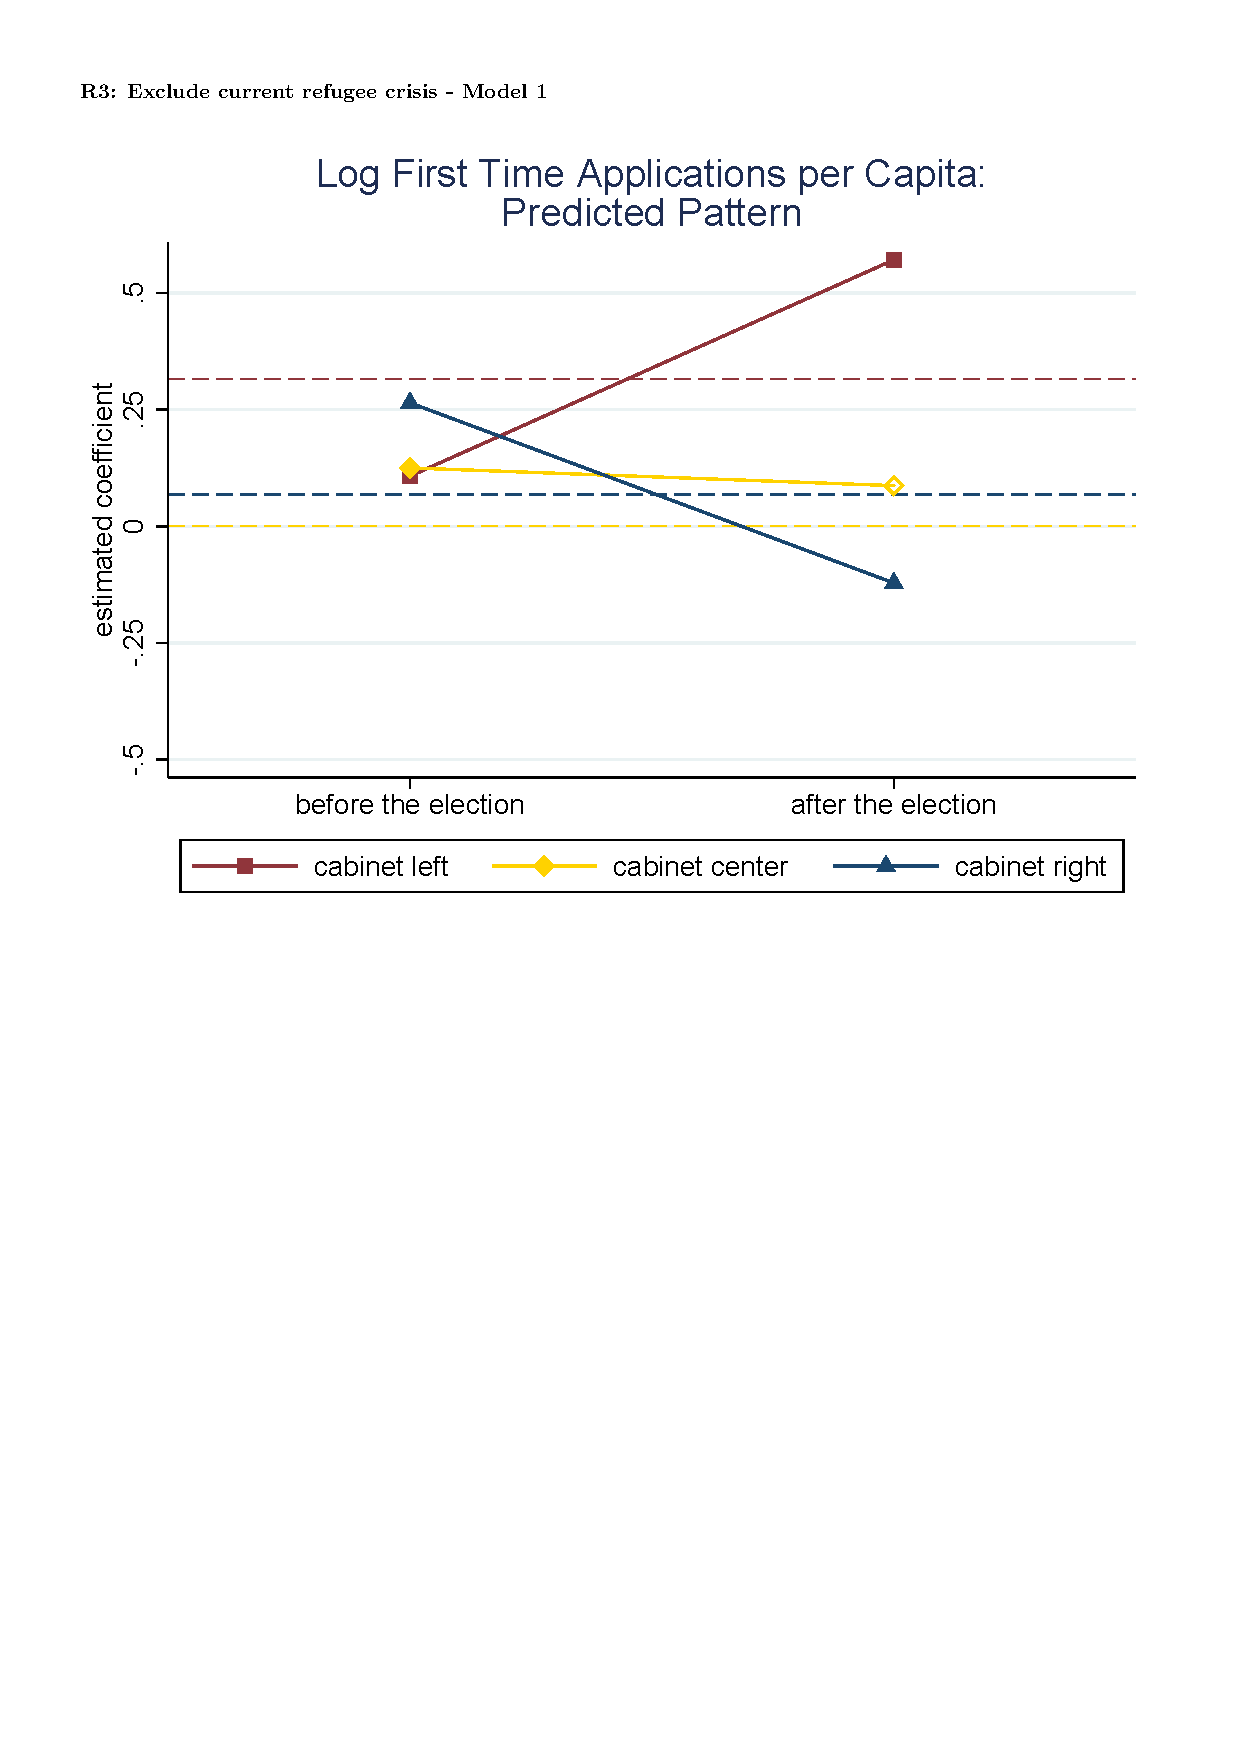
\includegraphics[width=10cm]{graph1.pdf}
 \end{center}
\end{figure}
\end{frame}

\begin{frame}{Asylum applications, quarterly}
\begin{figure}[tb]
\begin{center}
  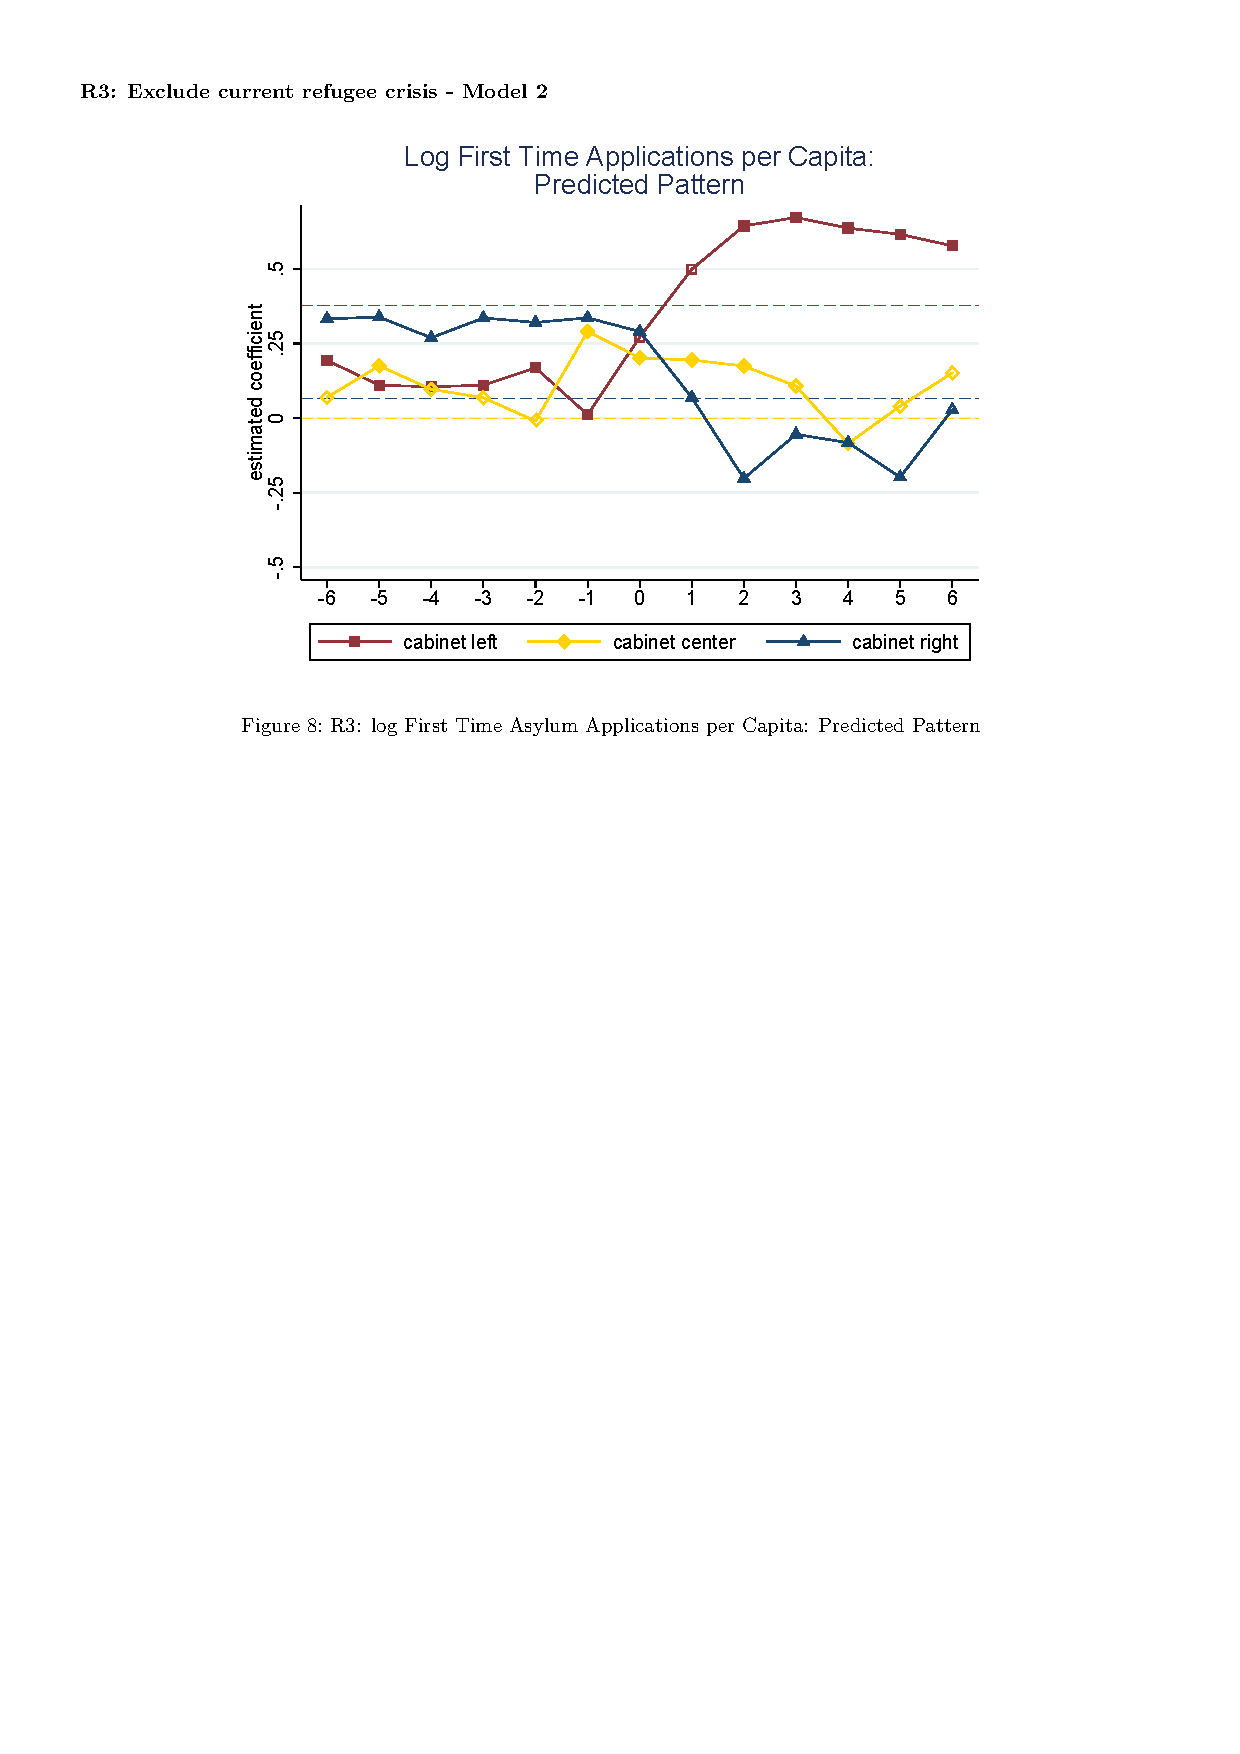
\includegraphics[width=12cm]{graph2.pdf}
 \end{center}
\end{figure}
\end{frame}

\begin{frame}{Asylum decisions, quarterly}
\begin{figure}[tb]
\begin{center}
  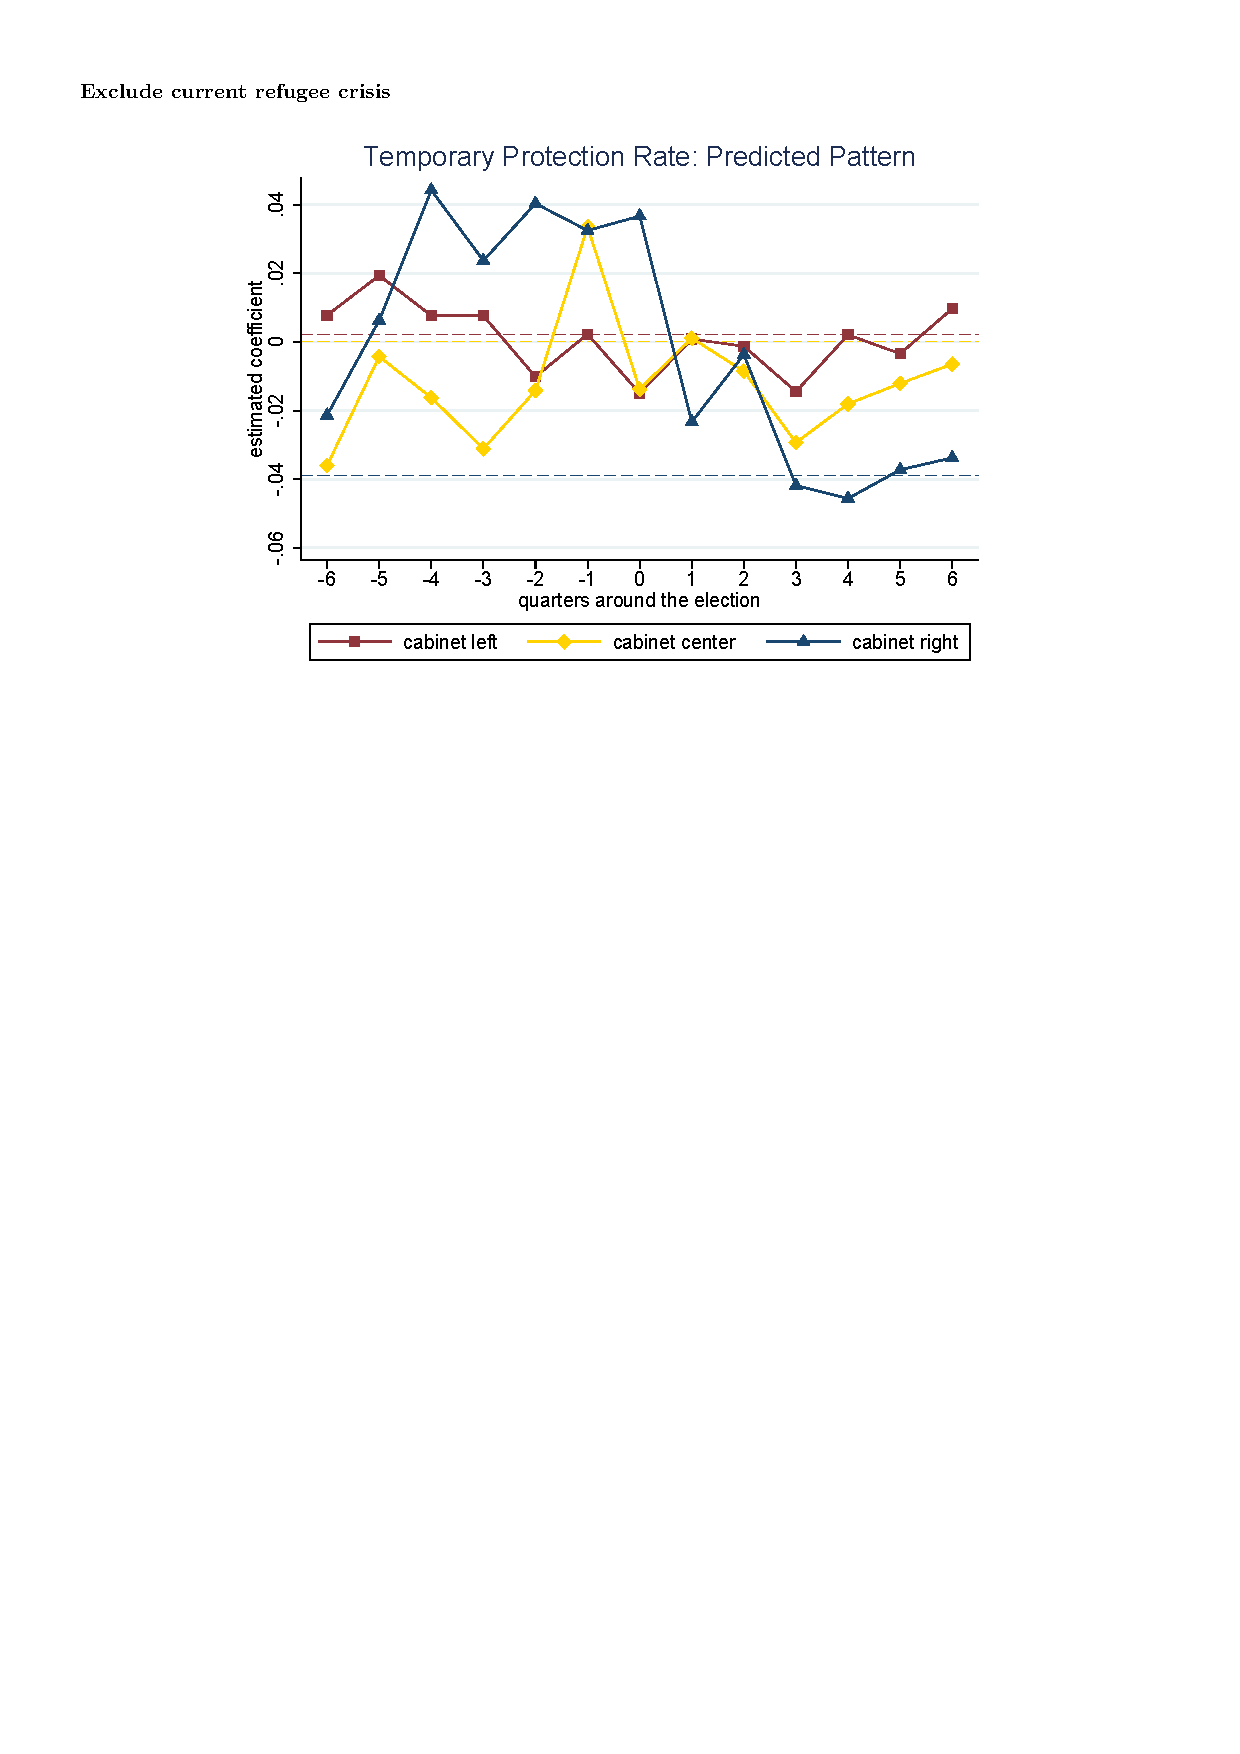
\includegraphics[width=12cm]{graph3.pdf}
 \end{center}
\end{figure}
\end{frame}


\section{Robustness}
%--------------------------------------------------------------------------------------------------%
	\begin{frame}{Robustness}
\begin{itemize}
\item Current refugee crisis excluded
\item Cabinets' stance on immigration policy  
\item All countries and years available included 
\item Only 4/5 quarters around the election dependent, etc. variable
\item Analysis by subgroups based on religion and language
\end{itemize}
	\end{frame}


%--------------------------------------------------------------------------------------------------%
	\begin{frame}
\Large
\begin{center}
\textbf{{Thank you for your attention!}}
\end{center}
\normalsize
	\end{frame}

\end{document}


	\begin{frame}{Asylum applications: Interaction effects}
\vspace{-2ex}
\begin{table}
\caption{First-time asylum applications per capita (log)}
\centering
\begin{threeparttable}
\begin{tabular}{l*{6}{c}}
\hline\hline
                    &\multicolumn{1}{c}{(1)}&\multicolumn{1}{c}{(2)}&\multicolumn{1}{c}{(3)}\\
& left & center & center\\
\hline
Before          &    -0.208***         &    0.125*         & 0.196***         \\
                                        &   (0.0410)         &   (0.0533)         &   (0.0409)         \\
After         &    0.255***&    00870  &    -0.189***\\
                                        &  (0.0391)         &  (0.0524)         &  (0.0572)         \\
\hline
Observations & 9432 & 9432 & 9432 \\
\hline
\hline
\end{tabular}
\end{threeparttable}
\end{table}
	\end{frame}
